\subsection{NFV Architecture}

The goal of NFV  is to be able to run network services traditionally hosted in specialized hardware in virtualized resources like virtual machines and containers. This gives the necessary flexibility for realizing use-cases discussed above.  The following figure shows the reference architecture of a typical NFV deployment. 

\begin{figure}
	\centering
	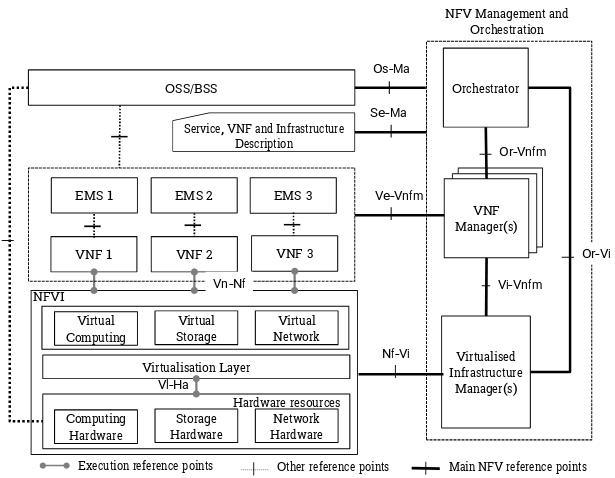
\includegraphics[width=0.9\textwidth]{nfv_ref_architecture}
	\label{fig:figure5}
	\caption{ETSI NFV Reference Architecture}
\end{figure}
